\documentclass{article}
\usepackage{hyperref}
\usepackage{amsmath}
\usepackage{amssymb}
\usepackage{pgfplots}
\usepackage{float}
\usepackage{todonotes}
\usepackage{tikz}
\usepackage[shortlabels]{enumitem}

\renewcommand{\Re}{\mathbb{R}}
\newcommand{\Li}{\mathcal{L}}
\newcommand{\Ex}{\mathbb{E}}
\renewcommand{\Pr}{\mathbb{P}}
\newcommand{\Hy}{\mathcal{H}}
\newcommand{\sign}{\text{sign}}
\newcommand{\error}{\text{error}}

\newcommand\bigO[1]{
    \ensuremath{\mathcal{O}\left(#1\right)}
    }

\newcommand{\sigmoidPlot}{
    
    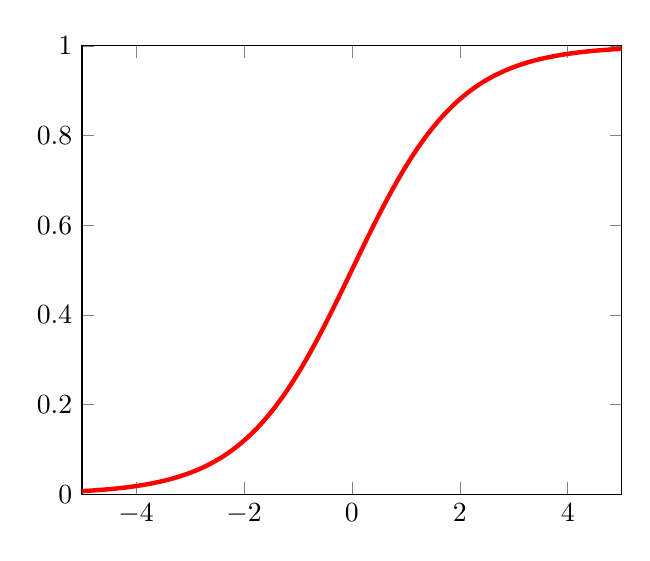
\begin{tikzpicture}
        \begin{axis}[xmin=-5, xmax=5, ymin=0, ymax=1, samples=150]
        \addplot[red, ultra thick] {1/(1+exp(-x))};
        \end{axis}
    \end{tikzpicture}
    
    }

\usetikzlibrary{positioning, calc}
\usetikzlibrary{arrows.meta}

\tikzstyle{circlebox}=[circle,thick,draw=black!75,minimum size=8mm]
\tikzstyle{inputnode}=[circlebox, draw=blue!75]
\tikzstyle{hiddennode}=[circlebox, draw=orange!75]
\tikzstyle{outputnode}=[circlebox, draw=orange!75]
\tikzstyle{simplebox}=[rectangle,thick,draw=black!75,
fill=black!20,minimum size=4mm]
\tikzstyle{textbox}=[rectangle,thick,minimum size=4mm,draw=black!0,
fill=black!0]
\tikzstyle{halfvdistance}=[yshift=-0.7cm]
\tikzstyle{abovebetween}=[xshift=-2.7mm]
\tikzstyle{edgepath} = [-Latex,->,shorten >=1pt,-stealth,semithick, rounded 
corners=5pt]

\def \nodedv {0.735cm}
\def \nodedh {0.65cm}

\tikzset{
    between/.style args={#1 and #2}{
        at = ($(#1)!0.5!(#2)$)
    }
}

\begin{document}
    \section{Subjects}
    \begin{itemize}
        \item Bagging
        \item Boosting
    \end{itemize}
    
    \section{Notes}
    
    \subsection{Decision trees}
    Decision trees simply split the feature space into a set of rectangles, and 
    then fit a simple model (e.g. a constant) in each one.
    
    So one might say that, we we take some input $x$ and ask a series of 
    questions. Is $x < 21$? Then go down the left path of the tree of 
    questions. So decision trees are very simple to understand but gain are 
    also very expressive. One of the major benefits of decision trees, is that 
    they are very easy to read and understand. It's very easy to look at it and 
    figure out what questions it asks and how much does it weigh that question 
    (e.g. what pixels does it look at to understand what the image is, what 
    pixels are ``important'').
    
    If we just look at a very simple form of decision trees, i.e. binary trees 
    then things will be a bit simpler. Then every question is of the form ``if 
    this then go left, otherwise go right'' so every node in the tree is a 
    single dividing line in the feature space. If we look at tree where the 
    values of the regions are constant, then we can predict the value of 
    some input $x$ as follows:
    \begin{equation*}
        h(x)=\sum_{\text{regions } r.} 1_{[x\in r]} \cdot c_r(x)
    \end{equation*}
    That is the constant value of the region that $x$ is in.
    
    \subsubsection{Growing a regression tree}
    Using the binary regression tree described earlier, with constant region 
    values, we will then describe how to grow a regression tree (learn).
    
    Given some input of $N$ observations $(x_i,y_i)$ for $i=1,2,\dots,N$ with 
    $x_i = (x_{i1}, x_{i2},\dots,x_{id})$ and $y_i$ being the label or the 
    ``true'' value, we then need to figure out how to approximate $y$ for some 
    unknown $x$ outside of the training set. The algorithm then needs to decide 
    on the splitting variables and split points, as well as the topology of the 
    tree.
    
    Suppose we have a partition into $M$ regions $R_1, R_2, \dots, R_M$ and we 
    model the response as mentioned earlier:
    \begin{equation*}
        h(x)=\sum_{\text{regions } r}1_{[x\in r]} \cdot c_r(x)
    \end{equation*}
    As usual with regression, we can use the squared error measure: $(h(x_i) 
    -y_i)^2$ to evaluate our performance. Then, we can easily see that the best 
    constant for region $R_m$ is simply the average of $y_i$ which ended up in 
    region $R_m$, because least squares measure punishes distance the target. 
    I.e. one point which is off by $2$ is punished more than two points that 
    are off by $1$, and thus the mean is the smallest distance on average:
    \begin{equation*}
        \hat{c}_m=\frac{1}{|D|}\sum_{(x,y) \in D}1_{[x\in r]} \cdot y
    \end{equation*}
    
    Now, actually finding the best partition of the feature space into the 
    $R_m$ optimal regions is, in general, computationally infeasible. Thus, we 
    will proceed with a greedy approximation algorithm.
    
    Consider some splitting variable $j$ and splitting point $s$, we can then 
    define the pair of half-planes:
    \begin{equation*}
        R_1(j,s)=\{X|X_j \leq s\} \text{ and } R_2(j,s)=\{X|X_j > s\}
    \end{equation*}
    Note here that the point $X$ can be any point in the feature space and is 
    not necessarily a point from $D$.
    
    We then seek to find the splitting variable $j$ and split point $s$ that 
    solve:
    \begin{equation*}
        \min_{j,s}\left[\min_{c_1}\left[\sum_{x_i\in 
        R_1(j,s)}(y_i-c_1)^2\right] + \min_{c_2}\left[\sum_{x_i \in 
        R_2(j,s)}(y_i-c_2)^2\right]\right]
    \end{equation*}
    
    If we use the mean, as mentioned earlier, we can simplify this to:
    \begin{equation*}
    \min_{j,s}\left[ \left(\sum_{x_i \in R_1(j,s)} (y_i - \hat{c}_1)^2 \right) 
    + \left(\sum_{x_i \in R_2(j,s)} (y_i - \hat{c}_2)^2 \right) \right]
    \end{equation*}
    Or, stated differently:
    \begin{equation*}
    \min_{j,s}\left[ \left(\sum_{(x, y) \in D, x_j \leq s} (y - \hat{c}_1)^2 
    \right) + \left(\sum_{x,y \in D, x_j > s} (y_i - \hat{c}_2)^2 \right) 
    \right]
    \end{equation*}
    For each splitting variable $j$, we can simply pick $s$ as the midpoints 
    between two $x_j$ values, which results in $|D| - 1$ different split-points 
    to consider.
    
    Now that we know how to compute the ``best'' split, we simply follow the 
    following greedy algorithm:
    \begin{itemize}
        \item Select best ``split'' variable $j$, and the split-point $s$
        \item Make a new node in the tree with $(j,s)$ (i.e. a new split)
        \item Make a child for each new region (outcome of testing $j$)
        \item Split the training examples up between the two regions
        \item Call recursively on the new children (the new regions)
        \item Stop when done
    \end{itemize}
    
    \subsubsection{Size of the tree}
    How large should the tree become? If we make it too large, we might 
    overfit. Too small and we might not capture the structure of the data 
    properly.
    
    Tree size is a hyper-parameter, and it should be chosen adaptively based on 
    the data. We could, for example, stop if the decrease in error drops below 
    some is under some threshold. This is fairly short-sighted however, as a 
    bad split at some level might result in a crucial split later on.
    
    The usual strategy is to grow a large tree $T_0$ and stop it when the size 
    of the nodes (i.e. how many data-points we have for each node) drops below 
    some set threshold (e.g. $5$) and then pruning this tree.
    
    One way to prune the tree, is to simply compute the accuracy gained by 
    removing on some validation set and greedily deleting the splits that 
    increases accuracy the most. Repeating this as long as it helps.
    
    Limiting the size of the tree is the same as regularizing for decision 
    trees. So variance will go down and bias will go up etc.
    
    \subsection{Classification trees}
    For regression trees, we used the squared error impurity measure $Q_m(T)$:
    \begin{equation*}
        Q_m(T)=\frac{1}{N_m}\sum_{x_i \in R_m}(y_i - \hat{c}_m)^2
    \end{equation*}
    Where $N_m = |\{x_i | x_i\in R_m\}|$ If the target is a classification 
    outcome, taking values $1,2,\dots,K$, then this measure is not suitable.
    
    If we let $\hat{p}_{mk}$ be the proportion of observations that had class 
    $k$ in node $m$. We can then predict the class of points in region $m$ to 
    have class $k(m)=\arg\max_k \hat{p}_{mk}$, i.e. the majority class in 
    region $m$. Then, different measures of $Q_m(T)$ of node impurity includes 
    the following:
    \begin{description}
        \item[Misclassification error (0-1 Loss)]
        \begin{equation*}
            \frac{1}{N_m} \sum_{(x,y) \in R_m}1_{[k(m) \neq y]} = 1- 
            \hat{p}_{mk(m)}
        \end{equation*}
        \item[Gini index]
        \begin{equation*}
            \sum_{k\neq k'} \hat{p}_{mk}\hat{p}_{mk'} = 
            \sum_{k=1}^{K}\hat{p}_{mk}(1-\hat{p}_{mk})
        \end{equation*}
        \item[Cross-entropy]
        \begin{equation*}
            - \sum_{k=1}^{K} \hat{p}_{mk} \log \hat{p}_{mk}
        \end{equation*}
    \end{description}
    
    \subsubsection{Why binary splits?}
    We can represent multiway splits by a series of binary splits (e.g. a 
    tertiary split can be represented by two binary splits) so we don't lose 
    generality. Furthermore, multiway splits split the data too quickly, so we 
    are left with too little information at the lower levels.
    
    \subsection{Ensemble methods}
    Decision trees have a high variance, just one data-point can completely 
    change the outcome of the tree. When we did the pruning and size-limitation 
    we sought to decrease the variance (through regularization). Another option 
    for reducing variance is ensemble methods.
    
    \subsubsection{Bootstrapping datasets}
    Bootstrapping is a general tool for assessing statistical accuracy. Suppose 
    we have our data-set $D$ as before. The basic idea is then to pick random 
    points from this such that we have $B$ different data-sets $D_i$ that each 
    have a random selection of points from $D$ (which may be overlapping). We 
    can use these data-sets $D_i$ as ``independent'' data-sets. This method is 
    often used to measure statistics like variance, confidence bounds, std.err. 
    etc. in other, more statistical oriented, domains.
    
    \subsubsection{Bagging}
    Bagging uses bootstrapped data-sets in order to improve on our predictions. 
    What we do in bagging (bootstrap aggregation) is simply to get our $B$ 
    bootstrapped data-sets $D_i$, train our model on all the different 
    data-sets producing $h_1,\dots,h_B$ (our ensemble of models). We can then 
    perform predictions by doing a majority vote (for classification) or 
    returning the mean of the predictions.
    \begin{equation*}
        h_{\text{bag}}(x)=\frac{1}{B}\sum_{i=1}^{B} h_i(x)
    \end{equation*}
    
    
    
\end{document}